\documentclass{article}
\usepackage[utf8]{inputenc}

\usepackage[dvipsnames]{xcolor}
\usepackage{tikz,lipsum,lmodern}
\usepackage[most]{tcolorbox} % Package to make colored boxes

\usepackage{tikz}
\usepackage[top=1in,bottom=1in,right=1in,left=1in]{geometry} %Unit Circle

\usepackage{amsmath} % for the equation* environment
\usepackage{tabularx}
\usepackage{multirow} % Required for multirows
\usepackage{booktabs} % For prettier tables
\usepackage{siunitx} % Required for alignment
\usepackage{pgfplots}
\usepackage{pst-plot}
\usepackage{hyperref}
\pgfplotsset{compat = newest}
\sisetup{
  round-mode          = places, % Rounds numbers
  round-precision     = 2, % to 2 places
}

\title{Fishbowl Notes}
\author{Tiffany Pham}
\date{30 November 2022}

\begin{document}

\maketitle

\section*{Unit 1 - Right Triangle Trig}

\section*{Unit 2 - Non-Right Triangles}
\subsection{Law of Sines}
\begin{displaymath}
    \frac{{\sin A}}{a} = \frac{{\sin B}}{b} = \frac{{\sin C}}{c}
\end{displaymath}


\subsection{Law of Cosines}


\section*{Unit 3 - Angles and Rotation}

\section*{Unit 4 - Unit Circle Trig}
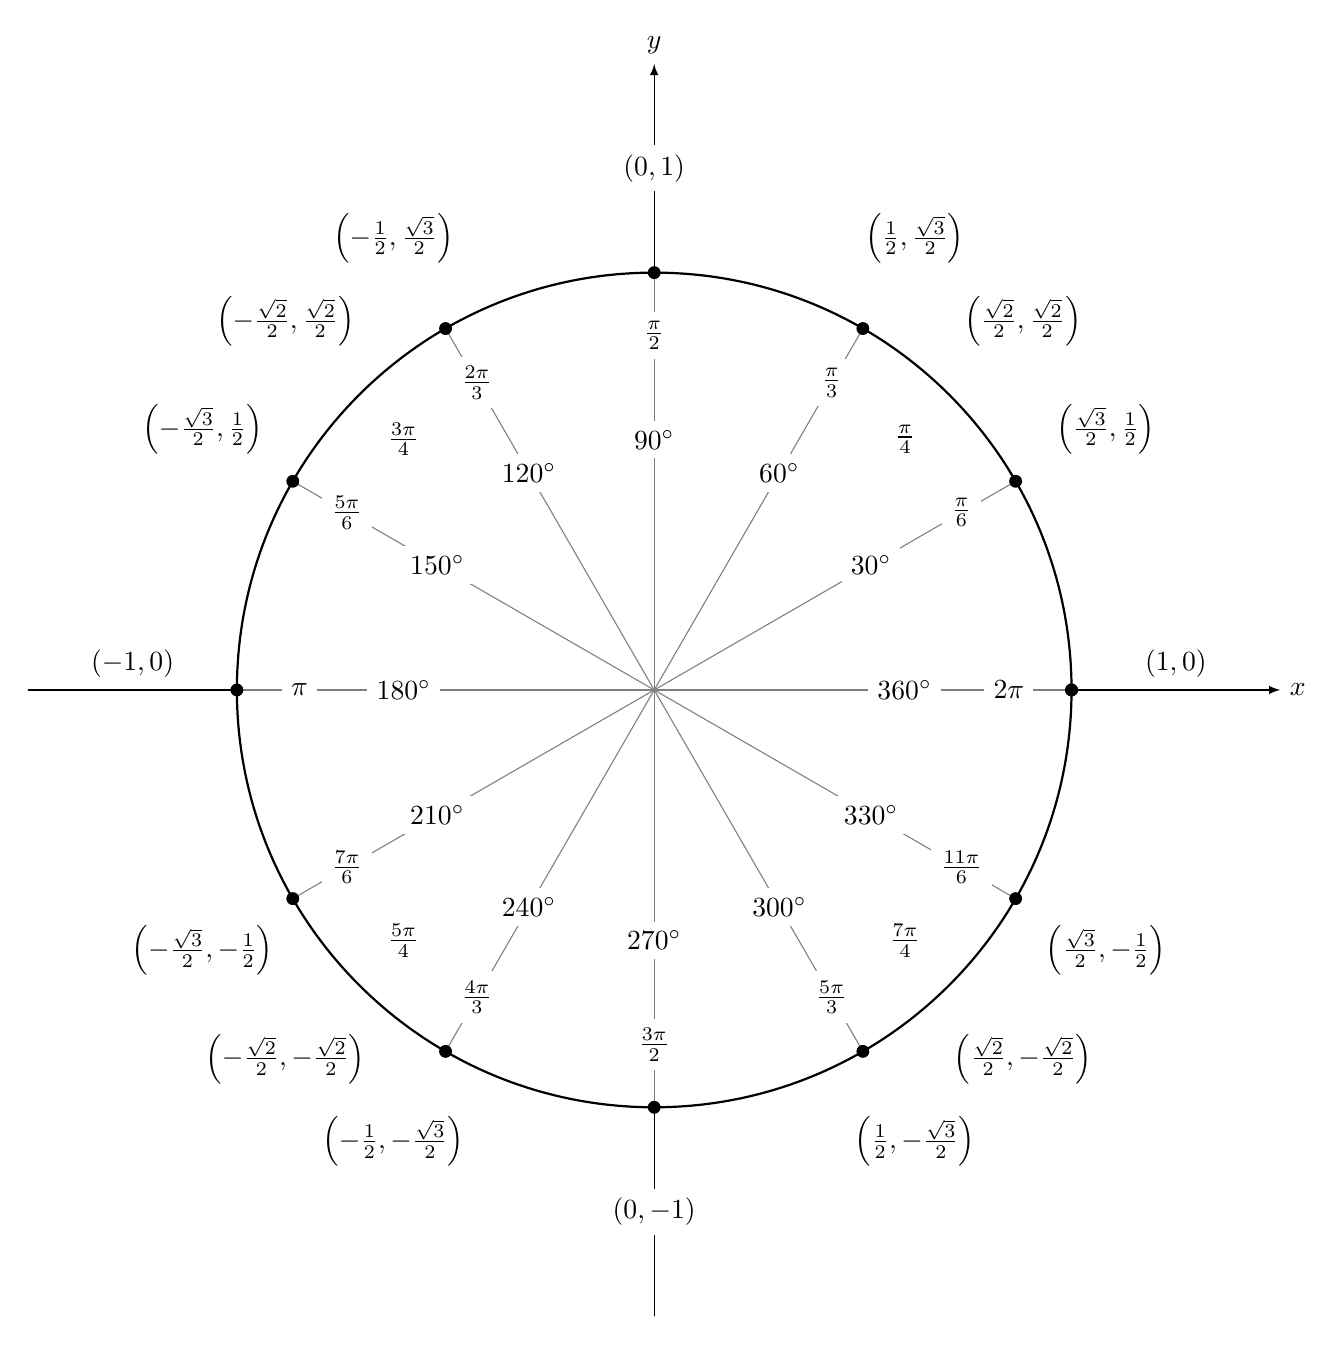
\begin{tikzpicture}[scale=5.3,cap=round,>=latex]
        % draw the coordinates
        \draw[->] (-1.5cm,0cm) -- (1.5cm,0cm) node[right,fill=white] {$x$};
        \draw[->] (0cm,-1.5cm) -- (0cm,1.5cm) node[above,fill=white] {$y$};

        % draw the unit circle
        \draw[thick] (0cm,0cm) circle(1cm);

        \foreach \x in {0,30,...,360} {
                % lines from center to point
                \draw[gray] (0cm,0cm) -- (\x:1cm);
                % dots at each point
                \filldraw[black] (\x:1cm) circle(0.4pt);
                % draw each angle in degrees
                \draw (\x:0.6cm) node[fill=white] {$\x^\circ$};
        }

        % draw each angle in radians
        \foreach \x/\xtext in {
            30/\frac{\pi}{6},
            45/\frac{\pi}{4},
            60/\frac{\pi}{3},
            90/\frac{\pi}{2},
            120/\frac{2\pi}{3},
            135/\frac{3\pi}{4},
            150/\frac{5\pi}{6},
            180/\pi,
            210/\frac{7\pi}{6},
            225/\frac{5\pi}{4},
            240/\frac{4\pi}{3},
            270/\frac{3\pi}{2},
            300/\frac{5\pi}{3},
            315/\frac{7\pi}{4},
            330/\frac{11\pi}{6},
            360/2\pi}
                \draw (\x:0.85cm) node[fill=white] {$\xtext$};

        \foreach \x/\xtext/\y in {
            % the coordinates for the first quadrant
            30/\frac{\sqrt{3}}{2}/\frac{1}{2},
            45/\frac{\sqrt{2}}{2}/\frac{\sqrt{2}}{2},
            60/\frac{1}{2}/\frac{\sqrt{3}}{2},
            % the coordinates for the second quadrant
            150/-\frac{\sqrt{3}}{2}/\frac{1}{2},
            135/-\frac{\sqrt{2}}{2}/\frac{\sqrt{2}}{2},
            120/-\frac{1}{2}/\frac{\sqrt{3}}{2},
            % the coordinates for the third quadrant
            210/-\frac{\sqrt{3}}{2}/-\frac{1}{2},
            225/-\frac{\sqrt{2}}{2}/-\frac{\sqrt{2}}{2},
            240/-\frac{1}{2}/-\frac{\sqrt{3}}{2},
            % the coordinates for the fourth quadrant
            330/\frac{\sqrt{3}}{2}/-\frac{1}{2},
            315/\frac{\sqrt{2}}{2}/-\frac{\sqrt{2}}{2},
            300/\frac{1}{2}/-\frac{\sqrt{3}}{2}}
                \draw (\x:1.25cm) node[fill=white] {$\left(\xtext,\y\right)$};

        % draw the horizontal and vertical coordinates
        % the placement is better this way
        \draw (-1.25cm,0cm) node[above=1pt] {$(-1,0)$}
              (1.25cm,0cm)  node[above=1pt] {$(1,0)$}
              (0cm,-1.25cm) node[fill=white] {$(0,-1)$}
              (0cm,1.25cm)  node[fill=white] {$(0,1)$};
    \end{tikzpicture}

\section*{Unit 5 - Graphing with Trig Functions}

\section*{Unit 6 - Modeling with Trig Functions}
\hfill \break
\subsection{Basic Equation}
\begin{displaymath}
    y=a\sin(bx-c)+d
\end{displaymath}

\hspace{3in} or
\begin{displaymath}
    y=a\cos(bx-c)+d
\end{displaymath}

\vspace{2mm}
\subsection{Advanced Equation?}
\begin{displaymath}
    y=A*\sin(B(x-H))+K
\end{displaymath}

\hspace{3in} or
\begin{displaymath}
    y=A*\cos(B(x-H))+K
\end{displaymath}

\vspace{4.9in}
\subsection{Sinusoidal Function Key} %beginning of explanation table
\hfill \break
\begin{tcolorbox}[colback=green!5!white,
                colframe=green!75!black]
  \begin{displaymath}
    y=A*\sin(B(x-H))+K
\end{displaymath}

\hspace{3in} or
\begin{displaymath}
    y=A*\cos(B(x-H))+K
\end{displaymath}
  \tcblower
\textbf{A} = \textbf{Amplitude} =   \[
    \frac{\text{max y - min y}}{\text{2}}
  \]
\textbf{Amplitude} can also never be negative so, it will be the absolute value of the answer.

\hfill \break
\textbf{B} = The number of cycles the graph completes in an interval of from 0 to 2$\pi$ or 360º. The value B affects the \textbf{period}.

\hfill \break
\textbf{Period} = 
\begin{displaymath}
    (\text{min }x-\text{max }x)*2
\end{displaymath}
\hfill \break
Once you get the \textbf{period}, you will plug it in for:
\begin{displaymath}
    \frac{2\pi}{\text{period}}
\end{displaymath}
This will give you the \textbf{B} value
\hfill \break

\textbf{H} = The horizontal shift (or phase shift) of a graph.
\hfill \break

To find \textbf{H} for \textbf{cos}, you will always use the max x-value unless its negative, then you will use the minimum x-value.
\hfill \break

To find \textbf{H} for \textbf{sine}, you can do: \[
    \frac{\text{period}}{\text{4}}+ \text{the smaller }x \text{ coord}
  \]

\textbf{K} = \textbf{midline}. To find the \textbf{midline} if you are given the \textit{\textbf{min y value}}:
\begin{displaymath}
    \text{min }y\text{ value}+\text{amplitude}=\text{midline}
\end{displaymath}
If you are given the \textit{\textbf{max y value}}, then:
\begin{displaymath}
    \text{max }y\text{ value}-\text{amplitude}=\text{midline}
\end{displaymath}

\textbf{NOTE}:
\hfill \break
If you are given a \textbf{maximum} and \textbf{minimum} point, then we will know the \textbf{h value} of \textbf{cos}.
\hfill \break

If you are given \textbf{2 midlines}, then we will know the \textbf{h value} of \textbf{sine}.
\end{tcolorbox} %ending of explanation table

\section{Example Problems} %Start of example problem table
\begin{tcolorbox}[
  colback=Magenta!5!white,
  colframe=Magenta!75!black,
  title={\centering Example 1 \textbf{(Creating Sine and Cosine Equations)}}]
\begin{center}
    Write TWO equations to fit the data. One as a sine equation in the form
\end{center}
\begin{displaymath}
    y=A*\sin(B(x-H))+K
\end{displaymath}
\begin{center}
    and the other as a cosine equation in the form
\end{center}
\begin{displaymath}
    y=A*\cos(B(x-H))+K
\end{displaymath}
\begin{center}
    Points = \textbf{Minimum (0.08602, 1.5337)}
    and
    \textbf{Maximum (1.2903, 4.61420)}
\end{center}
\end{tcolorbox}
\hfill \break First, find the \textbf{amplitude}:
\[
    Amp=\frac{\text{max y - min y}}{2}=\frac{4.6142-1.5337}{2}=1.54025
  \]
Then find the \textbf{period}:
\begin{center}
    \textit{Period} = (min \textit{x} - max \textit{x})2 = (0.08602 - 1.2903)2 = -2.40856=\textit{ (period)}
\end{center}
If the \textbf{period} is \textbf{negative}, then just make it \textbf{positive} since it is the \textbf{absolute value} of the number. So it would be 2.40856.
\hfill \break
\begin{displaymath}
    2.40856\text{ }->\frac{2\pi}{\textit{b}}=\frac{2\pi}{2.40856}=2.608689552=\textit{b}
\end{displaymath}
\hfill \break
To find the \textbf{H} value for \textbf{cos}, you will just have to take the \textbf{maximum x-value}. Unless it is negative, then you will use the \textbf{minimum x-value}.
\hfill \break
So \textbf{H} for \textbf{cos} is:
\begin{center}
    \textbf{\textit{H}=}1.29\text{ (for\textit{\textbf{ cosine}})}
\end{center}
\hfill \break
To find the \textbf{H} value for \textbf{sine} is:
\hfill \break
\begin{displaymath}
    \frac{\text{period}}{4}+\text{smaller x coordinate}=h
\end{displaymath}
\hfill \break
So \textbf{H} for \textbf{sine} is:
\hfill \break
\begin{displaymath}
    \frac{2.40856}{4}=0.60214+0.08602=0.68816\text{ (for \textit{\textbf{sine}})}
\end{displaymath}
Lastly, we will need to find \textbf{K}, which is:
\begin{displaymath}
    \text{min y value}+\text{amplitude}=\text{midline}=1.5337+1.54025=3.07=\textit{midline/K}
\end{displaymath}
\hfill \break
Now that we have found all the required information, we can make the \textbf{cosine} and \textbf{sine} equations. We can start with the \textbf{cosine} equation since we were given a \textbf{minimum} and \textbf{maximum} point.

\hfill \break
Equation for \textbf{cosine}:
\begin{displaymath}
    y=1.54\cos(2.6(x-1.29))+3.07
\end{displaymath}
\hfill \break
Equation for \textbf{sine}:
\begin{displaymath}
    y=-1.54\sin(2.6(x-.68816))+3.07
\end{displaymath}

\begin{tcolorbox}[
  colback=Magenta!5!white,
  colframe=Magenta!75!black,
  title={\centering Homework}]
mathhhhh oui oui
\end{tcolorbox}

\begin{tcolorbox}[
  colback=Magenta!5!white,
  colframe=Magenta!75!black,
  title={\centering Homework}]
math, math and more math
\end{tcolorbox}

\begin{tcolorbox}[
  colback=Magenta!5!white,
  colframe=Magenta!75!black,
  title={\centering Homework}]
mathhhh. noe
\end{tcolorbox}
%Remember to write starting points to show how to do shifts


\end{document}
